\documentclass[11pt]{article}
\usepackage[a4paper,left=3.0cm,right=2.0cm,top=1.0cm,bottom=2.0cm]{geometry}
\usepackage{graphicx}
\usepackage[brazil]{babel}
\usepackage[utf8]{inputenc}
\usepackage{indentfirst}

\author{Luciano Serafim de Souza\\Ramon Santos}
\title{Universidade Federal Rural de Pernambuco\\Unidade Acadêmica de Garanhuns\\Curso de Bacharelado em Ciência da Computação\vspace{5mm}\\ {\large Sistema de gerenciamento de locação de veículos do setor de transportes da Unidade Acadêmica de Garanhuns}}

\begin{document}

\frenchspacing

\maketitle

\begin{abstract}
O SLV - Sistema de Locação de Veículos tem o objetivo de automatizar o processo de solicitação de veículos na Unidade Acadêmica de Garanhuns - UFRPE. Foi inicialmente pensado pelo professor Luciano Souza como solução para o setor de transportes da unidade, uma vez que todo o processo de locação e acompanhamento de locação de veículos para visitas didáticas técnicas e de pesquisa são feitas de forma manual através de planilhas eletrônicas. 
\end{abstract}
\section{Introdução}
O sistema de gerenciamento de locação de veículos consiste em um ambiente onde os usuários poderão solicitar ao setor de transporte a reserva de veículos para realizar atividades referentes a visitação ou pesquisa.

A proposta do sistema é que o usuário tenha a disposição um ambiente WEB e dois aplicativos escritos na linguagem para dispositivos mobile, ANDROID.

O ambiente WEB vai dispor de dois serviços, área administrativa e área do usuário. Ambos terão acesso por meio de cadastro prévio e criação de um login e senha. 

As aplicações para dispositivos mobile vão ser utilizadas pelos usuários (Professores e Técnicos) e motoristas. Poderão ser realizadas solicitações de veículos, acompanhamento de solicitações, cancelamento e preenchimento de relatório de viagem respectivamente.

O sistema terá quatro tipos de usuário, 'Administrador' (Funcionário responsável pelo Setor de Transportes), 'Técnico' (Servidores em geral da Instituição), 'Professor Pesquisador (Professores que desenvolvam atividades de pesquisa e que precise locar carro destinado para esse fim) e 'Professor' (Professor que não desenvolve atividade de pesquisa, mas precisará de veículos para desenvolver atividades de práticas e visitação). Esses últimos serão cadastrados por Administradores levando-se em conta os dados necessários para a correta identificação dos mesmos, incluindo-se documentos e dados institucionais. Como citado acima ambos os tipos de usuário possuirão credenciais para login no sistema.

Após o login, o usuário terá acesso à sua área onde poderá preencher um formulário para a solicitação de veículos. Ao término da solicitação será gerado um número de protocolo e o pedido seguirá para análise pelo setor responsável. O usuário poderá verificar o status de seus pedidos em andamento buscando-os pelo protocolo ou através da visualização dos pedidos associados a seu nome ou matrícula, havendo também a possibilidade de cancelamento do pedido.

Será possível aos Administradores consultar todos os dados do sistema. Caberá a eles a inclusão ou exclusão de veículos e usuários do sistema, assim como a alteração de status dos pedidos. Para definir um status como 'Concluído', será necessário a entrada dos dados quantitativos referentes à viagem, incluindo o número de quilômetros rodados e quantidade de combustível consumido.

O objetivo deste projeto é o de automatizar a alocação de veículos na instituição, facilitando a atividade que hoje vem sendo feita através de planilhas eletrônicas e formulários preenchidos a cunho.

\section{MER - Modelo Entidade Relacionamento}
Pode-se ver abaixo o Modelo Entidade Relacionamento. Aqui são descritos em forma de diagrama as entidades envolvidas e os relacionamentos entre elas.
\begin{center}
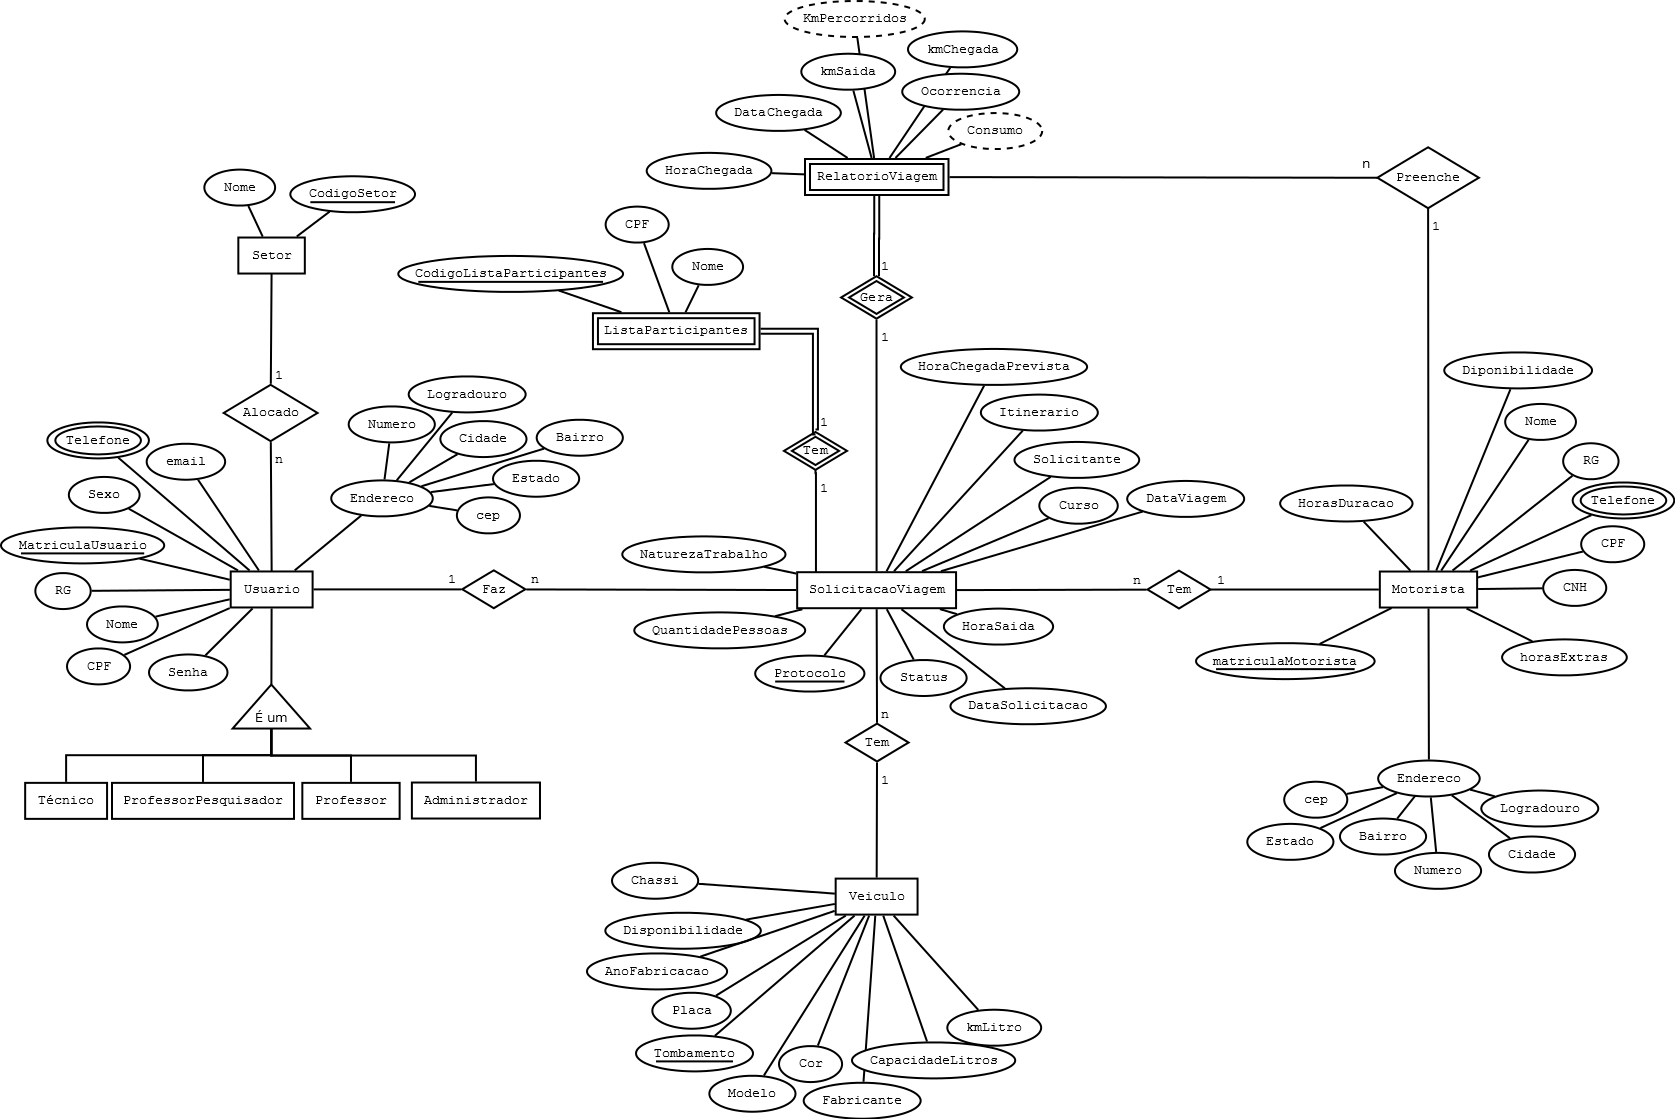
\includegraphics[scale=0.3]{esquema.png}
\end{center}   

\subsection{Modelo Esquema Relacional}

\subsubsection{Entidades regulares}
\begin{itemize}

\item setor(\underline{codigoSetor}, nome)

\item Motorista(\underline{cpfMotorista}, rgMotorista, cnh, nome, sexo, telefoneCelular, telefoneResidencial, senha, orgaoExpeditor, disponibilidade, logradouro, numero, cidade, bairro, estado, cep, email, horasExtras)

\item veiculo(\underline{codigoVeiculo}, tombamento, fabricante, modelo, cor, placa, anoFabricacao, chassi, disponibilidade, capacidadeLitros, kmLitro)
\end{itemize}

\subsubsection{Entidades Fracas}
\begin{itemize}

\item relatorioViagem(\underline{protocolo}, cpfMotorista, kmSaida, kmChegada, dataChegada, horaChegada, ocorrencia)

\item ListaParticipantes(\underline{protocolo}, cpfParticipante, nome)

\end{itemize}

\subsubsection{Relacionamentos 1:1}
\begin{itemize}

\item Como a entidade fraca ,RelatorioViagem e ListaParticipantes, também tem cardinalidade 1:1 e na regra anterior já foi tradado nesse passo não será necessário faze-lo.
\end{itemize}

\subsubsection{Relacionamentos 1:n(Que não envolvem entidades fracas)}
\begin{itemize}

\item usuario(\underline{cpfUsuario}, codigoSetor, nome, rgUsuario, orgaoExpeditor, telefoneCelular, telefoneResidencial, senha,
email, sexo, logradouro, numero, cidade, bairro, estado, cep)

\item solicitacaoViagem(\underline{protocolo}, solicitante, horaSaida, horaChegadaPrevista, dataViajem, naturezaTrabalho, quantidadePessoas, status, curso, itinerario, DataSolicitacao, cpfUsuario,  codigoVeiculo, cpfMotorista)

\end{itemize}

\subsubsection{Relacionamentos n:m}
Não existe relacionamento n:m.

\subsubsection{Atributos multivalorados}

Por conveniência decidiu-se não utilizar de atributos multivalorados.

\subsubsection{Especialização e Generalização}

Como existe quatro tipo de usuários do sistema (técnico, professor, professor pesquisador e administrador) optamos por criar um atributo (identificador) que pode receber um dos quatro tipos de usuários.

\begin{itemize}

\item usuarios(\underline{cpfUsuario}, codigoSetor, identificador, nome, rgUsuario, telefoneCelular, telefoneResidencial, orgaoExpeditor, senha,
email, sexo, logradouro, numero, cidade, bairro, estado, cep)

\end{itemize}

\section{Normalização}
Dado que o processo de modelagem para o esquema er foi eficaz, a normalização não foi necessária.

\section{Esquemas definitivos}
\begin{itemize}

\item \textbf{usuarios}(\underline{cpfUsuario}, codigoSetor, identificador, nome, rgUsuario, telefoneCelular, telefoneResidencial, orgaoExpeditor, senha,
email, sexo, logradouro, numero, cidade, bairro, estado, cep)

\item \textbf{solicitacaoViagem}(\underline{protocolo}, solicitante, horaSaida, horaChegadaPrevista, dataViajem, naturezaTrabalho, quantidadePessoas, status, curso, itinerario, DataSolicitacao, cpfUsuario,  codigoVeiculo, cpfMotorista)

\item \textbf{veiculo}(\underline{codigoVeiculo}, tombamento, fabricante, modelo, cor, placa, anoFabricacao, chassi, disponibilidade, capacidadeLitros, kmLitro)

\item \textbf{relatorioViagem}(\underline{protocolo}, cpfMotorista, kmSaida, kmChegada, dataChegada, horaChegada, ocorrencia)

\item \textbf{setor}(\underline{codigoSetor}, nome)

\item \textbf{Motorista}(\underline{cpfMotorista}, rgMotorista, cnh, nome, sexo, senha, telefoneCelular, telefoneResidencial, orgaoExpeditor, disponibilidade, logradouro, numero, cidade, bairro, estado, cep, email, horasExtras)

\item \textbf{ListaParticipantes}(\underline{protocolo}, cpfParticipante, nome)

\end{itemize}

\subsection{Diagrama de dados}

\begin{center}
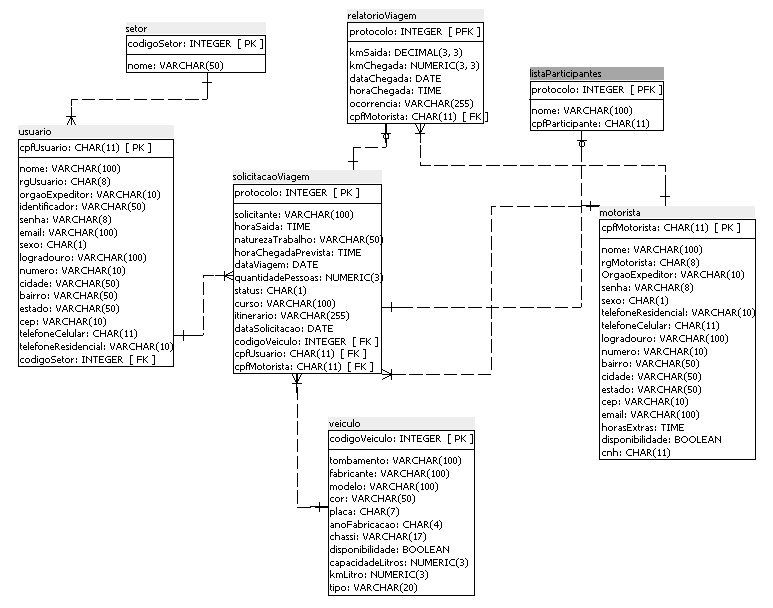
\includegraphics[scale=0.85]{diagramaDeDados.png}
\end{center}

\section{Scripts SQL}
\subsection{Mysql}
\begin{verbatim}

CREATE TABLE veiculo (
codigoVeiculo INT AUTO_INCREMENT NOT NULL,
tombamento VARCHAR(100) NOT NULL,
fabricante VARCHAR(100) NOT NULL,
modelo VARCHAR(100) NOT NULL,
cor VARCHAR(50) NOT NULL,
placa CHAR(7) NOT NULL,
anoFabricacao CHAR(4) NOT NULL,
chassi VARCHAR(17) NOT NULL,
disponibilidade BOOLEAN DEFAULT true NOT NULL,
capacidadeLitros NUMERIC(3) NOT NULL,
kmLitro NUMERIC(3) NOT NULL,
PRIMARY KEY (codigoVeiculo)
);


CREATE TABLE setor (
codigoSetor INT AUTO_INCREMENT NOT NULL,
nome VARCHAR(50) NOT NULL,
PRIMARY KEY (codigoSetor)
);


CREATE TABLE motorista (
cpfMotorista CHAR(11) NOT NULL,
nome VARCHAR(100) NOT NULL,
rgMotorista CHAR(8) NOT NULL,
OrgaoExpeditor VARCHAR(10) NOT NULL,
senha VARCHAR(8) NOT NULL,
sexo CHAR(1) NOT NULL,
telefoneResidencial VARCHAR(10),
telefoneCelular CHAR(11),
logradouro VARCHAR(100),
numero VARCHAR(10),
bairro VARCHAR(50),
cidade VARCHAR(50),
estado VARCHAR(50),
cep VARCHAR(10),
email VARCHAR(100),
horasExtras TIME,
disponibilidade BOOLEAN DEFAULT true,
cnh CHAR(11) NOT NULL,
PRIMARY KEY (cpfMotorista)
);


CREATE TABLE usuario (
cpfUsuario CHAR(11) NOT NULL,
nome VARCHAR(100) NOT NULL,
rgUsuario CHAR(8) NOT NULL,
orgaoExpeditor VARCHAR(10) NOT NULL,
identificador VARCHAR(50) NOT NULL,
senha VARCHAR(8) NOT NULL,
email VARCHAR(100),
sexo CHAR(1) NOT NULL,
logradouro VARCHAR(100),
numero VARCHAR(10),
cidade VARCHAR(50),
bairro VARCHAR(50),
estado VARCHAR(50),
cep VARCHAR(10),
telefoneCelular CHAR(11),
telefoneResidencial VARCHAR(10),
codigoSetor INT NOT NULL,
PRIMARY KEY (cpfUsuario)
);


CREATE TABLE solicitacaoViagem (
protocolo INT AUTO_INCREMENT NOT NULL,
solicitante VARCHAR(100) NOT NULL,
horaSaida TIME NOT NULL,
naturezaTrabalho VARCHAR(50) NOT NULL,
horaChegadaPrevista TIME NOT NULL,
dataViagem DATE NOT NULL,
quantidadePessoas NUMERIC(3) NOT NULL,
status CHAR(1) NOT NULL,
curso VARCHAR(100) NOT NULL,
itinerario VARCHAR(255) NOT NULL,
dataSolicitacao DATE NOT NULL,
codigoVeiculo INT NOT NULL,
cpfUsuario CHAR(11) NOT NULL,
cpfMotorista CHAR(11) NOT NULL,
PRIMARY KEY (protocolo)
);


CREATE TABLE relatorioViagem (
protocolo INT NOT NULL,
kmSaida DECIMAL(3,3) NOT NULL,
kmChegada NUMERIC(3,3),
dataChegada DATE,
horaChegada TIME,
ocorrencia VARCHAR(255) DEFAULT nd.,
cpfMotorista CHAR(11) NOT NULL,
PRIMARY KEY (protocolo)
);


CREATE TABLE listaParticipantes (
protocolo INT NOT NULL,
nome VARCHAR(100) NOT NULL,
cpfParticipante CHAR(11) NOT NULL,
PRIMARY KEY (protocolo)
);


ALTER TABLE solicitacaoViagem ADD CONSTRAINT veiculo_solicitacaoviagem_fk
FOREIGN KEY (codigoVeiculo)
REFERENCES veiculo (codigoVeiculo)
ON DELETE NO ACTION
ON UPDATE CASCADE;

ALTER TABLE usuario ADD CONSTRAINT setor_usuario_fk
FOREIGN KEY (codigoSetor)
REFERENCES setor (codigoSetor)
ON DELETE NO ACTION
ON UPDATE CASCADE;

ALTER TABLE solicitacaoViagem ADD CONSTRAINT motorista_solicitacaoviagem_fk
FOREIGN KEY (cpfMotorista)
REFERENCES motorista (cpfMotorista)
ON DELETE NO ACTION
ON UPDATE CASCADE;

ALTER TABLE relatorioViagem ADD CONSTRAINT motorista_relatorioviagem_fk
FOREIGN KEY (cpfMotorista)
REFERENCES motorista (cpfMotorista)
ON DELETE NO ACTION
ON UPDATE NO ACTION;

ALTER TABLE solicitacaoViagem ADD CONSTRAINT usuario_solicitacaoviagem_fk
FOREIGN KEY (cpfUsuario)
REFERENCES usuario (cpfUsuario)
ON DELETE NO ACTION
ON UPDATE CASCADE;

ALTER TABLE listaParticipantes ADD CONSTRAINT solicitacaoviagem_listaparticipantes_fk
FOREIGN KEY (protocolo)
REFERENCES solicitacaoViagem (protocolo)
ON DELETE NO ACTION
ON UPDATE CASCADE;

ALTER TABLE relatorioViagem ADD CONSTRAINT solicitacaoviagem_relatorioviagem_fk
FOREIGN KEY (protocolo)
REFERENCES solicitacaoViagem (protocolo)
ON DELETE NO ACTION
ON UPDATE CASCADE;
\end{verbatim}

\subsection{PostgreSQL}
\begin{verbatim}

CREATE TABLE public.veiculo (
codigoVeiculo INTEGER NOT NULL,
tombamento VARCHAR(100) NOT NULL,
fabricante VARCHAR(100) NOT NULL,
modelo VARCHAR(100) NOT NULL,
cor VARCHAR(50) NOT NULL,
placa CHAR(7) NOT NULL,
anoFabricacao CHAR(4) NOT NULL,
chassi VARCHAR(17) NOT NULL,
disponibilidade BOOLEAN DEFAULT true NOT NULL,
capacidadeLitros NUMERIC(3) NOT NULL,
kmLitro NUMERIC(3) NOT NULL,
CONSTRAINT codigoveiculo PRIMARY KEY (codigoVeiculo)
);

CREATE TABLE public.setor (
codigoSetor INTEGER NOT NULL,
nome VARCHAR(50) NOT NULL,
CONSTRAINT codigosetor PRIMARY KEY (codigoSetor)
);

CREATE TABLE public.motorista (
cpfMotorista CHAR(11) NOT NULL,
nome VARCHAR(100) NOT NULL,
rgMotorista CHAR(8) NOT NULL,
OrgaoExpeditor VARCHAR(10) NOT NULL,
senha VARCHAR(8) NOT NULL,
sexo CHAR(1) NOT NULL,
telefoneResidencial VARCHAR(10),
telefoneCelular CHAR(11),
logradouro VARCHAR(100),
numero VARCHAR(10),
bairro VARCHAR(50),
cidade VARCHAR(50),
estado VARCHAR(50),
cep VARCHAR(10),
email VARCHAR(100),
horasExtras TIME,
disponibilidade BOOLEAN DEFAULT true,
cnh CHAR(11) NOT NULL,
CONSTRAINT matriculamotorista PRIMARY KEY (cpfMotorista)
);


CREATE TABLE public.usuario (
cpfUsuario CHAR(11) NOT NULL,
nome VARCHAR(100) NOT NULL,
rgUsuario CHAR(8) NOT NULL,
orgaoExpeditor VARCHAR(10) NOT NULL,
identificador VARCHAR(50) NOT NULL,
senha VARCHAR(8) NOT NULL,
email VARCHAR(100),
sexo CHAR(1) NOT NULL,
logradouro VARCHAR(100),
numero VARCHAR(10),
cidade VARCHAR(50),
bairro VARCHAR(50),
estado VARCHAR(50),
cep VARCHAR(10),
telefoneCelular CHAR(11),
telefoneResidencial VARCHAR(10),
codigoSetor INTEGER NOT NULL,
CONSTRAINT matriculausuario PRIMARY KEY (cpfUsuario)
);

CREATE TABLE public.solicitacaoViagem (
protocolo INTEGER NOT NULL,
solicitante VARCHAR(100) NOT NULL,
horaSaida TIME NOT NULL,
naturezaTrabalho VARCHAR(50) NOT NULL,
horaChegadaPrevista TIME NOT NULL,
dataViagem DATE NOT NULL,
quantidadePessoas NUMERIC(3) NOT NULL,
status CHAR(1) NOT NULL,
curso VARCHAR(100) NOT NULL,
itinerario VARCHAR(255) NOT NULL,
dataSolicitacao DATE NOT NULL,
codigoVeiculo INTEGER NOT NULL,
cpfUsuario CHAR(11) NOT NULL,
cpfMotorista CHAR(11) NOT NULL,
CONSTRAINT protocolo PRIMARY KEY (protocolo)
);

CREATE TABLE public.relatorioViagem (
protocolo INTEGER NOT NULL,
kmSaida NUMERIC(3,3) NOT NULL,
kmChegada NUMERIC(3,3),
dataChegada DATE,
horaChegada TIME,
ocorrencia VARCHAR(255) DEFAULT nd.,
cpfMotorista CHAR(11) NOT NULL,
CONSTRAINT codigorelatorio PRIMARY KEY (protocolo)
);


CREATE TABLE public.listaParticipantes (
protocolo INTEGER NOT NULL,
nome VARCHAR(100) NOT NULL,
cpfParticipante CHAR(11) NOT NULL,
CONSTRAINT codigoparticipante PRIMARY KEY (protocolo)
);


ALTER TABLE public.solicitacaoViagem ADD CONSTRAINT veiculo_solicitacaoviagem_fk
FOREIGN KEY (codigoVeiculo)
REFERENCES public.veiculo (codigoVeiculo)
ON DELETE NO ACTION
ON UPDATE CASCADE
NOT DEFERRABLE;

ALTER TABLE public.usuario ADD CONSTRAINT setor_usuario_fk
FOREIGN KEY (codigoSetor)
REFERENCES public.setor (codigoSetor)
ON DELETE NO ACTION
ON UPDATE CASCADE
NOT DEFERRABLE;

ALTER TABLE public.solicitacaoViagem ADD CONSTRAINT motorista_solicitacaoviagem_fk
FOREIGN KEY (cpfMotorista)
REFERENCES public.motorista (cpfMotorista)
ON DELETE NO ACTION
ON UPDATE CASCADE
NOT DEFERRABLE;

ALTER TABLE public.relatorioViagem ADD CONSTRAINT motorista_relatorioviagem_fk
FOREIGN KEY (cpfMotorista)
REFERENCES public.motorista (cpfMotorista)
ON DELETE NO ACTION
ON UPDATE NO ACTION
NOT DEFERRABLE;

ALTER TABLE public.solicitacaoViagem ADD CONSTRAINT usuario_solicitacaoviagem_fk
FOREIGN KEY (cpfUsuario)
REFERENCES public.usuario (cpfUsuario)
ON DELETE NO ACTION
ON UPDATE CASCADE
NOT DEFERRABLE;

ALTER TABLE public.listaParticipantes ADD CONSTRAINT solicitacaoviagem_listaparticipantes_fk
FOREIGN KEY (protocolo)
REFERENCES public.solicitacaoViagem (protocolo)
ON DELETE NO ACTION
ON UPDATE CASCADE
NOT DEFERRABLE;

ALTER TABLE public.relatorioViagem ADD CONSTRAINT solicitacaoviagem_relatorioviagem_fk
FOREIGN KEY (protocolo)
REFERENCES public.solicitacaoViagem (protocolo)
ON DELETE NO ACTION
ON UPDATE CASCADE
NOT DEFERRABLE;
\end{verbatim}

\section{Requisitos}
\subsection{Funcionais}
\subsubsection{Administrador}
\begin{enumerate}
\item Cadastrar: Responsável pela inserção de \textbf{Usuários}, \textbf{Motoristas}, \textbf{Veículos} e \textbf{Setores} no sistema.
\item Alterar: Responsável pela alteração nos dados de \textbf{Usuários}, \textbf{Motoristas}, \textbf{Veículos} e \textbf{Setores} no sistema.
\item Excluir: Responsável pela exclusão de \textbf{Usuários}, \textbf{Motoristas}, \textbf{Veículos} e \textbf{Setores} no sistema.
\item Gerenciar solicitações: Responsável pelo gerenciamento das solicitações de locação dos veículos. Aqui o administrador poderá atualizar o status da solicitação que passa por três níveis: Em análise, autorizada e finalizada.
\item Tempo limite: Nessa funcionalidade o sistema informará ao usuário a janela de tempo que terá que ser cumprida para a autorização da viagem. Caso o usuário não faça dentro do tempo estipulado a solicitação não será concluída.
\item *Relatórios: Aqui o administrador poderá gerar relatórios sobre os veículos, usuários, solicitações e motoristas. Nas etapas finais de implementação será definido quais relatórios e que tipo de informações conterão estes.
\end{enumerate}

\subsubsection{Usuário}
\begin{enumerate}
\item Solicitar veiculo: O usuário fará a solicitação do veículo informando data da viagem, quantidade de pessoas entre algumas outras. Baseado nestas informações o sistema vai liberar o veículo de acordo coma natureza da viagem e a quantidade de pessoas informadas. O usuário poderá solicitar o veículo tanto pelo sistema web como app para android.
\item Recuperar senha: Caso o usuário esqueça a sua senha de acesso, ele poderá recupera-la. . Ela estará presente no sistema web e no app android.
\item Acompanhar solicitação: Aqui os usuários poderão acompanhar o status de suas solicitações.
\item Cancelar solicitação: Aqui os usuários poderão cancelar suas solicitações informando o motivo do cancelamento.
\end{enumerate}

\subsubsection{Motorista}
\begin{enumerate}
\item Verificar viagem: Ao verificar o motorista receberá a solicitação onde ele está alocado naquele dia.
\item Modificar relatório: Aqui o motorista poderá fazer alterações no relatório da solicitação da viagem.
\end{enumerate}

\subsubsection{Gerais}
\begin{enumerate}
\item Login: Responsável pelo controle do acesso dos usuários ao sistema. Ela estará presente no sistema web e no app android.
\end{enumerate}

\section{Ferramentas}
Serão utilizadas as seguintes ferramentas para o desenvolvimento do projeto:
\begin{itemize}
\item IDE Eclipse Kepler
\item Banco de Dados PostgreSQL
\item SGBD: phppgAdmin, pgAdmin III
\item Framework gráfico Primefaces
\item Servidor de aplicação Tomcat 7
\item Sistema de versionamento: git, github
\item Produção de relatório: TexMaker
\item UML: Dia - Diagram
\item Google drive
\item SQL Power Architect: Desenho do diagrama de dados e geração do script sql
\item Cronograma: Gantter.com
\end{itemize}
\end{document}
